\documentclass{article}
% translate with >> pdflatex -shell-escape <file>

% This file is used as unit test for pgfplots, copyright by Christian Feuersaenger.
% 
% See
%   http://pgfplots.sourceforge.net/pgfplots.pdf
% for pgfplots.
%
% Any required input files (for <plot table> or <plot file> or the table package) can be downloaded
% at
% http://www.ctan.org/tex-archive/graphics/pgf/contrib/pgfplots/doc/latex/
% and
% http://www.ctan.org/tex-archive/graphics/pgf/contrib/pgfplots/doc/latex/plotdata/

\usepackage{pgfplots}
\pgfplotsset{compat=1.3}

\pagestyle{empty}

\def\DoPlot{%
  \addplot+[no marks] expression[domain=1e1:1e5] { x^(.3) * (1 + 1e3*x^(-1)) / (1 + .5e3*x^(-1.3)) };
}

\begin{document}


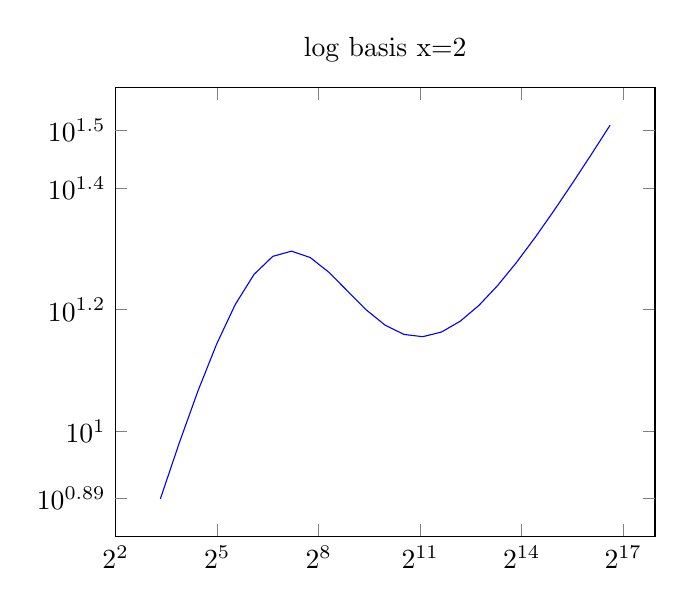
\begin{tikzpicture}
  \begin{loglogaxis}[log basis x=2,title={log basis x=2},extra y ticks={7.76,31.3}]
    \DoPlot
  \end{loglogaxis}
\end{tikzpicture}
\end{document}
